\chapter{Proposed Method}

\providecommand{\methodcode}[1]{\code{#1}}

\section{Research Motivation and Design Rationale}

The proposed method, denoted \bmab{}, is designed as a budget-aware extension of the original \mpage{} framework. The central observation behind this thesis is that LLM-driven heuristic design is not only an optimization problem over generated programs, but also a resource-allocation problem. Each heuristic-generation, clustering, or optional reflection step consumes an LLM call, and therefore consumes time, money, and limited experimental budget. A method that produces high-quality heuristics only after many unproductive calls is less useful than a method that converts early calls into a strong heuristic Pareto front.

The original \mpage{} paper formulates automatic heuristic design for multi-objective combinatorial optimization problems (MOCOPs) as a Language Multi-Criteria Heuristic Design problem. It combines three important ingredients: a SEMO-style heuristic population, Pareto-Front-Grid (PFG) elite selection, and LLM-based semantic clustering of heuristic code \cite{ha2026mpage,laumanns2004semo}. This design is well motivated because it searches for a population of heuristics that trade off solution quality and runtime, rather than a single best heuristic. It also recognizes that code-level diversity is not equivalent to semantic diversity: two heuristics may be syntactically different but implement nearly identical search logic.

However, the baseline \mpage{} workflow allocates generation effort in a mostly predetermined manner. Each generation repeatedly selects elites with PFG, groups promising heuristics into semantic clusters, applies mutation or crossover prompts, evaluates the generated program, and updates the population. This loop is effective for maintaining semantic and objective-space diversity, but it does not explicitly learn which operator or which semantic region is producing the most useful heuristics under the current budget. The stopping condition is also naturally expressed in terms of iterations or sample counts, whereas practical LLM-based search is constrained by a finite number of API calls. Under a strict budget $B$, the system should therefore learn where to spend the remaining LLM calls instead of treating all operators and clusters as equally promising.

\bmab{} therefore keeps the productive heuristic-generation mechanisms of \mpage{} and replaces only the scheduling layer. In particular, the implementation preserves the original task templates, prompt taxonomy, secure evaluator, PFG-based population management, and LLM semantic clustering implementation. The new contribution is a two-level budgeted multi-armed bandit controller that decides which variation operator and which semantic cluster should receive each LLM call. This design follows a conservative research principle: the comparison against \mpage{} is made meaningful by reusing the same generation and evaluation substrate, while changing the decision policy that allocates budget.

\section{Problem Formulation}

\subsection{Inner Multi-Objective Combinatorial Optimization Problem}

Let $\mathcal{X}$ be a finite or discrete feasible set for a MOCOP, and let

\begin{equation}
  f(x) = \left(f_1(x), f_2(x), \ldots, f_M(x)\right), \qquad x \in \mathcal{X},
\end{equation}

where all objectives are minimized. For two feasible solutions $x_a,x_b \in \mathcal{X}$, $x_a$ Pareto-dominates $x_b$, written $x_a \prec x_b$, if

\begin{equation}
  f_i(x_a) \le f_i(x_b) \quad \forall i \in \{1,\ldots,M\},
  \qquad
  \exists j: f_j(x_a) < f_j(x_b).
\end{equation}

The Pareto front is the image of the non-dominated solution set in objective space. Its quality is commonly summarized by the hypervolume indicator $HV_r(\cdot)$ with respect to a reference point $r$ \cite{zitzler1999multiobjective,fonseca2006hv}. For a finite objective set $Y$ in a minimization problem, the hypervolume is the Lebesgue measure of the region dominated by the non-dominated points in $Y$ and bounded by $r$:

\[
  HV_r(Y)
  =
  \lambda\!\left(
    \bigcup_{y \in \mathrm{ND}(Y)}
    [y_1,r_1]\times \cdots \times [y_M,r_M]
  \right),
\]

where $\mathrm{ND}(Y)$ denotes the non-dominated subset and $\lambda(\cdot)$ denotes $M$-dimensional volume. A larger hypervolume means that the obtained Pareto approximation is both closer to the ideal region and more broadly spread across trade-offs. The benchmark evaluators in this thesis use this quantity as the inner solution-quality signal and execution time as the efficiency signal.

\subsection{Outer Heuristic-Design Problem}

Following the LMHD formulation in the original \mpage{} paper, a heuristic $h \in \mathcal{H}$ is treated as a program that maps the current SEMO archive to a new candidate solution:

\begin{equation}
  h : 2^{\mathcal{X}} \rightarrow \mathcal{X}, \qquad x' = h(A),
\end{equation}

where $A$ is the current archive of non-dominated solutions maintained by the inner solver. The evaluator assigns each generated heuristic a vector-valued score

\begin{equation}
  E(h) = \left(e_1(h), e_2(h)\right)
       = \left(-HV_{\text{inner}}(h), T(h)\right).
  \label{eq:heuristic-score}
\end{equation}

Equation~\ref{eq:heuristic-score} should be read as the interface between heuristic design and the inner solver. The LLM does not directly output a TSP tour, CVRP route, or knapsack solution. Instead, it outputs a heuristic program $h$. During evaluation, the inner SEMO-style solver repeatedly calls $h$ with its current archive $A$ and expects one candidate solution $x'$. The quality of $h$ is therefore determined indirectly by the Pareto archive that the inner solver obtains after running with that heuristic.

Here $HV_{\text{inner}}(h)$ is the hypervolume achieved by the solutions produced when $h$ is used inside the benchmark solver, and $T(h)$ is the measured runtime. More concretely, if the inner run using $h$ returns a non-dominated solution archive $A_h$, then $HV_{\text{inner}}(h)$ is computed from the objective vectors $\{f(x):x\in A_h\}$ using the task-specific reference point. This is the \emph{inner hypervolume}: it measures how good one generated heuristic is at solving the underlying combinatorial optimization task.

The first coordinate in $E(h)$ is negated because the outer population-management code is written as a minimization procedure. Thus, a heuristic with a larger inner hypervolume receives a smaller first score coordinate. The second coordinate is runtime, so smaller is also better. This score convention is implemented by the benchmark evaluators in the vendored MPaGE task modules.

At the outer level, the algorithm maintains a population $\mathcal{P}_t \subset \mathcal{H}$ of valid heuristics and aims to approximate the non-dominated set in the heuristic score space. Let $F_t = \{E(h): h \in \mathcal{P}_t\}$ be the outer heuristic front at step $t$. Given an LLM-call budget $B$, \bmab{} is optimized for two related criteria:

\begin{align}
  \max \; HV_{\text{outer}}(B)
  &= \max \; HV_r(F_B), \\
  \max \; \mathrm{AUBC}
  &= \max \; \frac{1}{B}\int_0^B HV_{\text{outer}}(b)\,db,
  \label{eq:aubc-objective}
\end{align}

subject to

\begin{equation}
  \sum_{t=1}^{T} c_t \le B.
\end{equation}

The quantity $HV_{\text{outer}}$ is the \emph{outer hypervolume}: it is computed over heuristic score vectors rather than over task solutions. A high outer hypervolume means that the final population contains useful trade-offs between inner solution quality and runtime, for example heuristics that achieve high inner HV quickly and heuristics that are slower but stronger. The final HV objective measures terminal population quality, while AUBC measures how rapidly the method converts budget into Pareto-front quality over the whole run. In the current experiments, the default cost model is call-based, i.e. one LLM request consumes one budget unit. The budget tracker also supports a token-labeled accounting mode, but the implemented main loop and reported experiments use fixed call costs.

\section{System Overview}

\bmab{} is organized as an adaptive orchestration layer around the MPaGE primitives. Figure~\ref{fig:bmab-llm-main} summarizes this data and control flow at the level of one complete iteration. The left side starts from the current heuristic population and applies Pareto Front Grid decomposition to identify an elite set of heuristics. The selected heuristics are then passed to the semantic clustering and bandit-selection stage. The selected operator--cluster decision controls which parents are sampled and whether mutation or crossover is used. The generated offspring heuristic is evaluated, converted into a scalar reward signal, and then inserted into the managed population through non-dominated sorting and crowding-distance truncation.

\begin{figure}[H]
  \centering
  
\includegraphics[width=0.98\linewidth]{bmab_llm_main.png}
  \caption{Iteration-level pipeline of the proposed framework. The figure shows how the current heuristic population is decomposed by Pareto Front Grid selection, grouped by LLM semantic clustering, controlled by operator and cluster bandits, transformed through mutation or crossover prompts, evaluated by the benchmark evaluator, converted into reward feedback, and finally managed through non-dominated sorting and diversity-preserving truncation.}
  \label{fig:bmab-llm-main}
\end{figure}

This figure is important because it separates the roles of generation, evaluation, and control. The proposed framework preserves MPaGE's prompt, evaluation, semantic clustering, and population-management components, while adding budget accounting and adaptive bandit control around them. The LLM is used only to produce or refine heuristic programs; it does not directly solve the benchmark instances. The evaluator executes the generated heuristic inside the inner multi-objective search process and returns a heuristic score. That score is then used in two ways: it updates the managed heuristic population and it becomes part of the reward signal observed by the bandit controller. Consequently, the proposed framework forms a closed-loop system: generated heuristics affect rewards, rewards affect future operator and cluster choices, and those choices determine how the remaining LLM-call budget is spent.

The implementation is centered in \methodcode{bmab\_llm.py}. The main supporting modules are summarized in Table~\ref{tab:method-modules}.

\begin{table}[H]
  \centering
  \caption{Main methodological modules in the implementation.}
  \label{tab:method-modules}
  \begin{tabular}{p{0.28\linewidth}p{0.62\linewidth}}
    \toprule
    Module & Methodological role \\
    \midrule
    \methodcode{bmab\_llm.py} & Main orchestrator. It owns the evolutionary loop, calls PFG selection, requests semantic clusters, selects bandit arms, samples offspring, computes rewards, and flushes the final population. \\
    \methodcode{budget.py} & Hard budget tracker. It stores total, remaining, and consumed budget and records a history entry for every charged LLM call. \\
    \methodcode{bandit.py} & Two-level adaptive scheduler: persistent operator UCB, per-generation cluster UCB, and Page--Hinkley drift detection. \\
    \methodcode{cluster\_manager.py} & Wrapper around MPaGE semantic clustering. It charges cluster calls, validates or repairs partitions, and computes cluster-quality priors. \\
    \methodcode{reward.py} & Scalar credit assignment for bandit learning, including HVI, final managed-population HV gain, diversity gain, rank smoothing, and invalid-code penalties. \\
    \methodcode{profiler.py} & Records budget-vs-HV curves, AUBC, budget history, bandit state, and population artifacts for analysis. \\
    \bottomrule
  \end{tabular}
\end{table}

\section{Components Inherited from MPaGE}

\bmab{} intentionally retains the core generative and evaluative substrate of \mpage{}. This inheritance is documented in the implementation materials and is visible in the vendored MPaGE subtree. The retained components are important because they isolate the proposed contribution to budget-aware scheduling rather than changing the benchmark, prompt templates, or evaluation logic.

\subsection{Population Representation and PFG Selection}

Each individual is represented as a Python function together with a natural-language algorithm description, evaluation score, sample time, and execution time. The population class inherited from MPaGE maintains a managed set of heuristics using non-dominated sorting and diversity-preserving truncation.

PFG selection partitions the two-dimensional heuristic objective space into grid cells. Let $P_t = \{E(h_i): h_i \in \mathcal{P}_t\}$ be the current score set. For each objective $j \in \{1,2\}$, define the ideal and nadir values

\begin{equation}
  z_j^{\ast} = \min_{h \in \mathcal{P}_t} e_j(h), \qquad
  z_j^{n} = \max_{h \in \mathcal{P}_t} e_j(h).
\end{equation}

With $K_j$ segments and a small margin $\sigma$, the grid width is approximately

\begin{equation}
  \Delta_j = \frac{z_j^{n} - z_j^{\ast} + \sigma}{K_j}.
\end{equation}

A heuristic is assigned to a grid index

\begin{equation}
  g_j(h)=\left\lfloor \frac{e_j(h)-z_j^{\ast}}{\Delta_j}\right\rfloor,
  \qquad
  G(h)=(g_1(h),g_2(h)).
\end{equation}

Within each occupied cell, non-dominated representatives are retained. The union of retained representatives forms the elite set used for reproduction. This mechanism is inherited from \mpage{} and is implemented in the vendored MPaGE population manager. In the current BMAB loop, the PFG-selected slice is used as a high-quality signal for parent weighting, while the wider managed population is made available to the clustering layer to avoid over-narrow clusters.

\subsection{LLM-Based Semantic Clustering}

The original \mpage{} paper argues that objective-space or syntax-only diversity is insufficient for heuristic design. Two code snippets can have different syntax but the same algorithmic logic, and two heuristics with similar performance may use distinct search strategies. MPaGE addresses this by prompting an LLM to group elite heuristics according to semantic and behavioral similarity.

Formally, for a candidate set $P=\{h_1,\ldots,h_n\}$, the clustering module returns

\begin{equation}
  \mathrm{SemClust}(P)=\{C_1,\ldots,C_K\},
\end{equation}

such that

\begin{equation}
  \bigcup_{k=1}^{K} C_k=P, \qquad C_i \cap C_j = \emptyset \; (i \ne j).
\end{equation}

The implementation calls the MPaGE cluster prompt through \methodcode{cluster\_manager.py}. If the LLM response is malformed, incomplete, or unavailable, the method falls back to singleton clusters. This design preserves semantic clustering when possible while ensuring that the evolutionary loop remains robust to LLM-format failures.

\subsection{Mutation and Crossover Prompt Families}

MPaGE defines a prompt taxonomy for initialization, mutation, and crossover. \bmab{} keeps this taxonomy. Initialization uses the I1 prompt to create zero-shot heuristics. Mutation uses M1 or M2 to modify a single parent from the selected cluster. Crossover uses E1 or E2 to combine one parent from the selected cluster with a second parent outside that cluster. Thus, BMAB preserves MPaGE's core semantic rule:

\begin{equation}
  \text{mutation} = \text{intra-cluster local refinement},
  \qquad
  \text{crossover} = \text{inter-cluster recombination}.
\end{equation}

The difference is not the prompt content but the policy that decides when a mutation or crossover prompt should be used, and which cluster should provide the parent.

\section{Hard Budget Model}

The LLM-call budget is treated as a first-class constraint. Let $B$ be the total budget and $b_t$ be the remaining budget before action $t$. Each LLM action has cost $c_t$, and the transition is

\begin{equation}
  b_{t+1} = b_t - c_t, \qquad b_t \ge c_t.
\end{equation}

If the system cannot afford an action, the action is not issued. The current implementation charges budget before the heuristic-generation call or cluster call is sent. This is important experimentally: invalid code, parsing failure, timeout, and non-improving offspring are still charged because the API resource has already been consumed.

In the call-based mode used by the reported experiments, Table~\ref{tab:budget-costs} lists the costs charged by the budget tracker.

\begin{table}[H]
  \centering
  \caption{Budget costs used by the current implementation.}
  \label{tab:budget-costs}
  \begin{tabular}{lc}
    \toprule
    Action & Cost \\
    \midrule
    Initialization call (I1) & $1$ \\
    Heuristic-generation call (M1/M2/E1/E2) & $1$ \\
    Semantic clustering call & $1$ \\
    Optional review/suggestion call & $1$ \\
    \bottomrule
  \end{tabular}
\end{table}

The budget state is recorded through \methodcode{BudgetTracker.history}, and the profiler later writes \methodcode{budget\_history.json}. This gives the experimental harness a direct account of how the budget was spent.

Figure~\ref{fig:bmab-llm-budget-manage} summarizes the two places where budget enters the method. On the left, the budget tracker gates expensive LLM actions: semantic clustering and mutation/crossover generation are allowed only when the remaining budget can pay for the call. On the right, the recorded sequence of consumed budget and outer hypervolume values forms the budget curve used to compute AUBC.

\begin{figure}[H]
  \centering
  
\includegraphics[width=0.98\linewidth]{bmab_llm_budget_manage.png}
  \caption{Budget management and AUBC measurement in the proposed framework. The budget tracker controls whether LLM semantic clustering or heuristic-generation calls can be issued, while the profiler records used budget and outer hypervolume so that the area under the budget curve can quantify budget efficiency.}
  \label{fig:bmab-llm-budget-manage}
\end{figure}

This view clarifies why budget control is not merely a stopping rule. A clustering call is useful only if it can guide later generation, and a generation call is useful only if its resulting heuristic can be evaluated and considered by the population manager. The budget tracker therefore shapes the exploration--exploitation process: early in the run, the scheduler can afford more exploratory cluster and operator choices; near the end, budget annealing reduces exploration pressure so that remaining calls are more likely to exploit productive regions. The AUBC measurement then evaluates this behavior over the whole trajectory rather than only at the final population.

\section{Two-Level Budgeted Bandit Scheduler}

\subsection{Why a Two-Level Scheduler is Needed}

A direct bandit over individual heuristics is not viable because the heuristic space is open-ended: every LLM call can create a previously unseen program. A direct persistent bandit over semantic cluster IDs is also problematic because clusters are reconstructed at each generation and their numeric labels are not stable across generations. \bmab{} therefore separates the adaptive decision into two levels:

\begin{enumerate}
  \item a persistent operator-level bandit over the stable action set $\mathcal{O}=\{\mu,\chi\}$, where $\mu$ denotes mutation and $\chi$ denotes crossover;
  \item a per-generation cluster-level bandit over arms $(k,o)$, where $k$ indexes one semantic cluster in the current generation and $o \in \mathcal{O}$ is the selected operator.
\end{enumerate}

This decomposition lets the method learn long-term operator utility while still adapting to the short-lived semantic cluster structure of the current population.

Figure~\ref{fig:bmab-llm-bandits} illustrates the corresponding feedback loop. The current managed population is clustered at the beginning of a generation. The persistent operator bandit provides a prior over mutation and crossover, while the generation-local cluster bandit creates arms that combine an operator with a semantic cluster. After an offspring heuristic is generated and evaluated, the reward computer sends feedback to both bandit levels. The Page--Hinkley state monitors the cluster-arm reward stream and can reset stale cluster statistics when reward behavior changes.

\begin{figure}[H]
  \centering
  
\includegraphics[width=0.82\linewidth]{bmab_llm_bandits.png}
  \caption{Feedback loop of the two-level bandit scheduler. The operator bandit learns persistent preferences over mutation and crossover, the cluster bandit selects generation-local operator--cluster arms, the reward computer updates both levels using observed heuristic quality, and Page--Hinkley drift detection can reset cluster-arm statistics when the local reward distribution becomes stale.}
  \label{fig:bmab-llm-bandits}
\end{figure}

The figure also shows how Final-HV reward and Hybrid reward fit into the scheduler. Both modes are implemented inside the reward computer and therefore affect the numerical feedback passed to the operator and cluster bandits. Final-HV reward gives credit when the managed archive improves after population management, whereas Hybrid reward combines that managed final-HV signal with immediate HVI feedback. The bandit mechanism is agnostic to the semantic meaning of the reward; it only observes scalar values. This separation is useful because the same scheduling machinery can compare different quality-signal designs while keeping the generation, evaluation, and archive-management pipeline fixed.

\subsection{Operator-Level UCB}

For each operator $o \in \mathcal{O}$, the operator bandit stores the number of pulls $n_o$, cumulative reward $S_o^R$, and cumulative cost $S_o^c$. Its empirical utility is reward per cost:

\begin{equation}
  \hat{\rho}_o = \frac{S_o^R}{\max(S_o^c,\varepsilon)}.
\end{equation}

The selected operator maximizes a UCB score:

\begin{equation}
  U_{\mathrm{op}}(o)
  =
  \hat{\rho}_o
  +
  c_{\mathrm{op}}
  \sqrt{\frac{2\log N_{\mathrm{op}}}{n_o}},
  \label{eq:operator-ucb}
\end{equation}

where $N_{\mathrm{op}}=\sum_{o' \in \mathcal{O}} n_{o'}$ and $c_{\mathrm{op}}$ controls exploration. The implementation initializes each operator with an optimistic prior count and prior reward, preventing division by zero and encouraging early exploration. This is implemented in \methodcode{bandit.py} by the \methodcode{OperatorBandit} class.

\subsection{Cluster-Level Budgeted UCB}

At the beginning of each generation, \methodcode{ClusterManager} returns a partition $\{C_1,\ldots,C_K\}$ and a quality prior $q_k$ for each cluster. At this point, $q_k$ can be understood as a scalar estimate of how promising cluster $C_k$ is before any new offspring are generated in the current generation; its formal front-aware definition is given in Section~\ref{sec:front-aware-priors}. The cluster bandit then creates arms $(k,o)$ for all clusters and operator labels. Each arm stores cumulative reward and cumulative cost, and its exploitation term is

\begin{equation}
  \hat{\rho}_{k,o}
  =
  \frac{S_{k,o}^R}{\max(S_{k,o}^c,\varepsilon)}.
\end{equation}

The cluster-level UCB score is

\begin{equation}
  U_{\mathrm{cl}}(k,o)
  =
  \hat{\rho}_{k,o}
  +
  c_{\mathrm{cl}}
  \alpha_t
  \sqrt{\frac{2\log N_{\mathrm{cl}}}{n_{k,o}}},
  \label{eq:cluster-ucb}
\end{equation}

where

\begin{equation}
  \alpha_t =
  \left(\frac{b_t}{B}\right)^{\gamma_b}
\end{equation}

when budget annealing is enabled, and $\alpha_t=1$ otherwise. The factor $\alpha_t$ decreases as the budget is exhausted, making the controller more exploitative near the end of the run. This directly addresses the finite-horizon nature of the task: late calls have little time to recover from risky exploration.

The cluster bandit is warm-started from both cluster quality and operator priors. Let $p_o$ be the softmax-normalized operator utility from the persistent operator bandit. The initial reward assigned to arm $(k,o)$ is proportional to

\begin{equation}
  r^{(0)}_{k,o} = \frac{1}{2}\left(q_k+p_o\right).
\end{equation}

This warm start transfers information from the persistent operator layer into the generation-local cluster layer without assuming that cluster IDs persist across generations.

\section{Front-Aware Cluster Priors}
\label{sec:front-aware-priors}

The semantic cluster partition identifies behavioral groups, but it does not by itself rank those groups. The current implementation therefore computes a front-aware prior for each cluster. For cluster $C_k$, define $S_k=\{E(h):h \in C_k\}$ and $S=\{E(h):h \in \mathcal{P}_t\}$. With outer reference point $r$, the hypervolume contribution of the cluster is

\begin{equation}
  \Delta HV_k
  =
  \max\left(0,\;HV_r(S)-HV_r(S\setminus S_k)\right).
\end{equation}

The heuristic scores in this section are the two-dimensional evaluator outputs $s=E(h)=(-HV_{\text{inner}}(h),T(h))$. Therefore, $s_1$ represents negated inner hypervolume and $s_2$ represents runtime. Because the first score coordinate is negative inner HV, a simple quality proxy for solution strength is

\begin{equation}
  I_k = \max\left(0,\;-\min_{s \in S_k} s_1\right),
\end{equation}

with a finite cap in the implementation to avoid an excessively large prior. A runtime proxy is defined as

\begin{equation}
  T_k = \frac{1}{1+\min_{s \in S_k} s_2}.
\end{equation}

The unnormalized prior is

\begin{equation}
  \tilde{q}_k = \Delta HV_k + 0.25 I_k + T_k,
\end{equation}

and the normalized prior used by the bandit is

\begin{equation}
  q_k = \frac{\tilde{q}_k}{\max_j \tilde{q}_j}
\end{equation}

when the denominator is positive. This design is implemented in \methodcode{cluster\_manager.py}. It is more aligned with the final outer-front objective than a one-dimensional score proxy because it rewards clusters that currently contribute to the heuristic Pareto front while still accounting for inner solution quality and runtime.

\section{Reward and Credit Assignment}

\subsection{Reward Components}

The reward function converts the outcome of one LLM generation call into a scalar signal for the two bandits. For a valid generated heuristic with score $s$, the reward is

\begin{equation}
  R(s)
  =
  w_q Q(s)
  +
  w_d \max(0,\Delta D)
  +
  w_r \mathrm{Rank}(s).
  \label{eq:reward}
\end{equation}

If the generated heuristic is invalid, cannot be parsed, fails evaluation, or returns a non-finite score, the reward is

\begin{equation}
  R(s) = -\lambda_{\mathrm{pen}}.
\end{equation}

The values used in the current implementation are $w_q=1.0$, $w_d=0.3$, $w_r=0.2$, and $\lambda_{\mathrm{pen}}=1.0$. These settings are exposed through the command-line interface for the weights and fixed in \methodcode{RewardComputer} for the penalty.

\subsection{Quality Signal}

Let $F$ be the set of valid population scores before the new candidate is inserted. The immediate hypervolume improvement is

\begin{equation}
  \mathrm{HVI}(s;F)
  =
  \max\left(0,\;HV_r(F\cup\{s\})-HV_r(F)\right).
\end{equation}

The implementation also computes a managed-population HV delta. Let $\mathrm{Manage}_N(\cdot)$ denote the same score-only survivor-selection logic used by the managed population with cap $N$. Then

\begin{equation}
  \Delta HV_{\mathrm{managed}}
  =
  \max\left(
    0,\;
    HV_r(\mathrm{Manage}_N(F\cup\{s\}))
    -
    HV_r(\mathrm{Manage}_N(F))
  \right).
  \label{eq:managed-hv}
\end{equation}

\subsubsection{Managed Archive Operator}

The operator $\mathrm{Manage}_N(\cdot)$ is the archive-management rule that connects a newly evaluated heuristic score to the final maintained population. It is not an additional optimizer over the underlying routing or knapsack instances. Instead, it operates at the outer heuristic-population level. Its input is a finite set of heuristic score vectors, such as the current valid score set $F$ or the temporary set $F\cup\{s\}$ obtained after adding a new candidate score $s$, together with a capacity limit $N$. Its output is a subset of at most $N$ score vectors that represents the managed archive used by the outer search.

The implementation follows the same survivor-selection logic as the population-management step used for the final heuristic population. First, only valid finite score vectors are considered. Invalid candidates, missing scores, and non-finite scores are handled before this step by assigning the invalid-code penalty, so they do not enter the managed archive. Second, the remaining score vectors are partitioned by fast non-dominated sorting under the minimization convention. A score vector is preferred if it is no worse in every objective and strictly better in at least one objective. Thus, dominated vectors are placed in later fronts and are selected only if the archive has remaining capacity after all better fronts have been accepted.

Third, $\mathrm{Manage}_N(\cdot)$ fills the archive front by front. If an entire non-dominated front fits within the remaining capacity, all scores in that front are kept. If the next front would exceed the capacity limit, the implementation computes crowding distance inside that front and keeps the scores with the largest crowding distances. Boundary scores in each objective receive infinite crowding distance, while interior scores receive a normalized distance based on neighboring objective values. This truncation rule preserves spread along the outer Pareto front when the archive must discard otherwise non-dominated alternatives. The implementation does not introduce a separate duplicate-removal criterion inside $\mathrm{Manage}_N(\cdot)$; identical or near-identical scores are treated as ordinary score vectors and are removed only if dominated or if the crowding-distance truncation excludes them.

This management step matters because the final reported heuristic population is capped. A candidate can increase the hypervolume of the uncapped temporary set $F\cup\{s\}$ but still be removed after $\mathrm{Manage}_N(\cdot)$ if it is dominated or if it is an interior point that loses the crowding-distance truncation. Conversely, a candidate that survives management, or that causes a better survivor set to be retained, can increase the hypervolume of the managed archive. For Final-HV reward, the two managed archives compared by Equation~\ref{eq:managed-hv} are

\begin{equation}
  A^-=\mathrm{Manage}_N(F),
  \qquad
  A^+=\mathrm{Manage}_N(F\cup\{s\}).
\end{equation}

The raw Final-HV quality signal is therefore $\max(0,HV_r(A^+)-HV_r(A^-))$, which is then normalized online as described below. This construction gives credit only to candidates whose contribution survives the same management rule that determines the final population. In other words, the bandit is not rewarded merely because a candidate briefly improves an uncapped archive; it is rewarded when the maintained archive after capacity control becomes better.

Both immediate HVI and managed HV delta can have very different numerical scales across tasks and across stages of the search. The implementation therefore normalizes them online by rolling maxima over a recent reward window. For reward event $t$, this can be written as

\begin{align}
  \widehat{\mathrm{HVI}}_t
  &=
  \frac{\mathrm{HVI}_t}
  {\max\left(\epsilon,\max_{\tau\in W_t}\mathrm{HVI}_\tau\right)},\\
  \widehat{\Delta HV}_{\mathrm{managed},t}
  &=
  \frac{\Delta HV_{\mathrm{managed},t}}
  {\max\left(\epsilon,\max_{\tau\in W_t}\Delta HV_{\mathrm{managed},\tau}\right)},
\end{align}

where $W_t$ denotes the recent rolling window and $\epsilon$ is a small positive floor used to avoid division by zero. Let $\widehat{\mathrm{HVI}}$ and $\widehat{\Delta HV}_{\mathrm{managed}}$ denote these normalized values. The two thesis-facing quality modes are then

\begin{equation}
  Q(s)=
  \begin{cases}
    \widehat{\Delta HV}_{\mathrm{managed}}(s;F),
    & \mathrm{mode}=\mathrm{final\_hv},\\
    \frac{1}{2}\widehat{\mathrm{HVI}}(s;F)
    +\frac{1}{2}\widehat{\Delta HV}_{\mathrm{managed}}(s;F),
    & \mathrm{mode}=\mathrm{hybrid}.
  \end{cases}
\end{equation}

Final-HV reward mode uses the normalized managed-population delta $\widehat{\Delta HV}_{\mathrm{managed}}$. It asks a strict question: after inserting the candidate, applying $\mathrm{Manage}_N(\cdot)$, and recomputing hypervolume on the capped survivor set, how much did the maintained population improve? This is a delta-HV-managed reward mode. Its reward is still computed after each evaluated candidate, but the candidate is credited only for the hypervolume improvement that survives archive management. This makes the signal directly aligned with the final reported heuristic population, because candidates that look useful locally but do not affect the capped survivor set receive little or no quality reward.

The drawback of this strict alignment is that the signal can become sparse, especially late in the search. As the managed archive improves, a new heuristic must do more than produce a locally non-dominated score; it must also survive capacity control and increase the hypervolume of the maintained archive. Many valid candidates therefore receive zero quality reward even though they contain some local information about promising regions of the outer score space.

Hybrid reward mode is introduced to reduce this sparsity while preserving the final-quality orientation of Final-HV reward. Its quality signal averages two normalized quantities: the immediate HVI term $\widehat{\mathrm{HVI}}$, which reacts to local expansion of the current uncapped score set, and the managed delta term $\widehat{\Delta HV}_{\mathrm{managed}}$, which checks whether the improvement survives archive management. The immediate term gives the bandit more frequent feedback during search, while the managed term prevents the reward from drifting away from the final capped-population objective.

The following example illustrates why immediate HVI and managed final-HV delta can assign different quality credit. Consider a two-objective minimization score space with reference point $r=(10,10)$ and managed population cap $N=2$. Let the current valid heuristic-score set already contain two boundary trade-off scores:

\begin{equation}
  F=\{a=(1,8),\; c=(8,1)\},
\end{equation}

and suppose that a newly generated heuristic receives score $x=(3,5)$. Here the points are heuristic scores, not inner problem solutions. The new score $x$ is non-dominated with respect to $F$ and expands the uncapped dominated region between the two boundary scores. Therefore its raw immediate improvement is positive:

\begin{equation}
  r_{\mathrm{HVI}}^{\mathrm{raw}}
  =
  HV_r(F\cup\{x\})-HV_r(F)
  =
  47-32
  =
  15.
\end{equation}

The immediate-HVI component of Hybrid reward uses the rolling-normalized version of this positive value. However, the managed reward asks a different question. Before inserting $x$, the capped management rule keeps only two survivors:

\begin{equation}
  \mathrm{Manage}_2(F)=\{a,c\}.
\end{equation}

In this example, all three scores in $F\cup\{x\}$ are non-dominated, but $a$ and $c$ are boundary trade-off points and receive the largest crowding-distance priority when the non-dominated front must be truncated to two points. The interior score $x$ is therefore discarded by $\mathrm{Manage}_2(F\cup\{x\})$, which still returns $\{a,c\}$. Consequently,

\begin{equation}
  r_{\mathrm{final}}^{\mathrm{raw}}
  =
  HV_r(\mathrm{Manage}_2(F\cup\{x\}))
  -
  HV_r(\mathrm{Manage}_2(F))
  =
  HV_r(\{a,c\})-HV_r(\{a,c\})
  =
  0.
\end{equation}

The example therefore has the following management sequence. First, the archive before insertion is $F=\{a,c\}$ and its managed form is unchanged, $A^-=\mathrm{Manage}_2(F)=\{a,c\}$. Second, the new candidate $x$ is evaluated and temporarily added, giving $F_{\mathrm{tmp}}=F\cup\{x\}$. Third, the temporary set has larger uncapped hypervolume, so the immediate-HVI component is positive. Fourth, $\mathrm{Manage}_2(F_{\mathrm{tmp}})$ applies the archive cap and keeps only the two boundary scores, returning $A^+=\{a,c\}$. Finally, because $HV_r(A^+)=HV_r(A^-)$, the raw Final-HV reward is zero. Figure~\ref{fig:immediate-final-reward-example} visualizes this distinction.

\begin{figure}[H]
  \centering
  \begin{minipage}{0.49\linewidth}
    \centering
    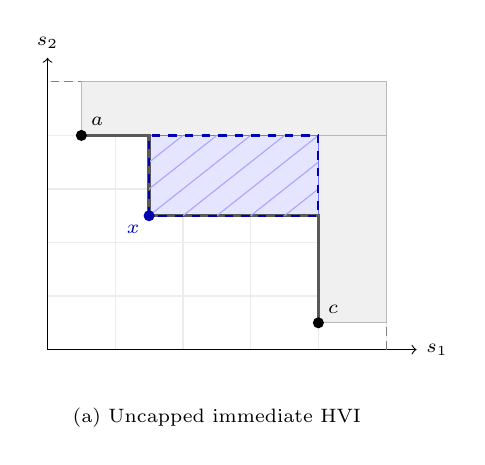
\begin{tikzpicture}[x=0.43cm,y=0.34cm,font=\scriptsize]
      \draw[step=2,gray!15] (0,0) grid (10,10);
      \draw[->] (0,0) -- (10.9,0) node[right] {$s_1$};
      \draw[->] (0,0) -- (0,10.9) node[above] {$s_2$};
      \draw[densely dashed,gray] (10,0) -- (10,10) -- (0,10);
      \node[gray!70!black,anchor=east] at (9.8,9.55) {$r=(10,10)$};
      \fill[gray!12] (1,8) rectangle (10,10);
      \draw[gray!55] (1,8) rectangle (10,10);
      \fill[gray!12] (8,1) rectangle (10,8);
      \draw[gray!55] (8,1) rectangle (10,8);
      \fill[blue!10] (3,5) rectangle (8,8);
      \draw[blue!55] (3,5) rectangle (8,8);
      \draw[very thick,gray!70!black] (1,8) -- (3,8) -- (3,5) -- (8,5) -- (8,1);
      \begin{scope}
        \clip (3,5) rectangle (8,8);
        \foreach \d in {-2,-1,...,8} {
          \draw[blue!35] (\d,5) -- ({\d+3},8);
        }
      \end{scope}
      \draw[blue!70!black,thick,dashed] (3,5) rectangle (8,8);
      \foreach \p/\name in {(1,8)/a,(8,1)/c} {
        \fill[black] \p circle (2pt);
        \node[above right] at \p {$\name$};
      }
      \fill[blue!70!black] (3,5) circle (2pt);
      \node[below left,blue!70!black] at (3,5) {$x$};
      \node[align=center] at (5,-2.55)
        {(a) Uncapped immediate HVI};
    \end{tikzpicture}
  \end{minipage}
  \hspace{0.01\linewidth}
  \begin{minipage}{0.49\linewidth}
    \centering
    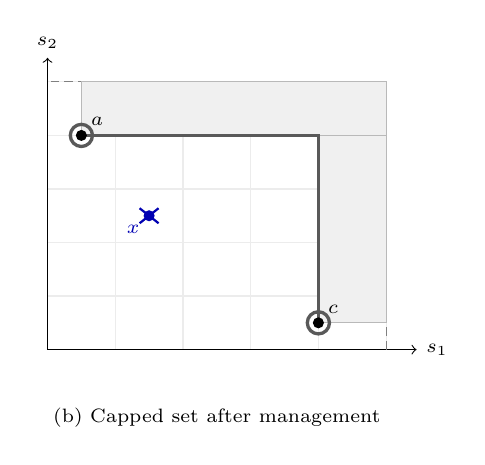
\begin{tikzpicture}[x=0.43cm,y=0.34cm,font=\scriptsize]
      \draw[step=2,gray!15] (0,0) grid (10,10);
      \draw[->] (0,0) -- (10.9,0) node[right] {$s_1$};
      \draw[->] (0,0) -- (0,10.9) node[above] {$s_2$};
      \draw[densely dashed,gray] (10,0) -- (10,10) -- (0,10);
      \node[gray!70!black,anchor=east] at (9.8,9.55) {$r=(10,10)$};
      \fill[gray!12] (1,8) rectangle (10,10);
      \draw[gray!55] (1,8) rectangle (10,10);
      \fill[gray!12] (8,1) rectangle (10,8);
      \draw[gray!55] (8,1) rectangle (10,8);
      \draw[very thick,gray!70!black] (1,8) -- (8,8) -- (8,1);
      \foreach \p/\name in {(1,8)/a,(8,1)/c} {
        \draw[gray!70!black,very thick] \p circle (4pt);
        \fill[black] \p circle (2pt);
        \node[above right] at \p {$\name$};
      }
      \fill[blue!70!black] (3,5) circle (2pt);
      \draw[blue!70!black,thick] (2.72,4.72) -- (3.28,5.28);
      \draw[blue!70!black,thick] (2.72,5.28) -- (3.28,4.72);
      \node[below left,blue!70!black] at (3,5) {$x$};
      \node[align=center] at (5,-2.55)
        {(b) Capped set after management};
    \end{tikzpicture}
  \end{minipage}
  \caption{Illustration of a case where immediate HVI and managed final-HV delta assign different quality credit. The neutral rectangles show the hypervolume already contributed by the existing boundary scores $a$ and $c$, while the blue rectangle marks only the additional HVI introduced by candidate $x$. The capped management operator with $N=2$ keeps the boundary scores $a$ and $c$ and removes $x$, so the managed-population hypervolume does not change.}
  \label{fig:immediate-final-reward-example}
\end{figure}

The example in Figure~\ref{fig:immediate-final-reward-example} shows the practical consequence. The immediate-HVI term reinforces candidates that make any immediate Pareto-front contribution, even if the contribution is interior and later removed by capacity control. Final-HV reward reinforces only candidates whose contribution survives population management. Hybrid reward uses both signals: it remains responsive to local front expansion but still gives explicit credit to improvements that affect the managed archive. In both retained reward modes, $Q(s)$ is only the quality component of the scalar bandit reward; the complete reward also includes the diversity and rank terms described below.

\subsection{Diversity and Rank Smoothing}

Pure HVI is often sparse: many valid offspring do not immediately expand the outer Pareto front. To provide a denser signal, \bmab{} adds rank and diversity terms. The cumulative diversity index used in the reward is the mean pairwise Euclidean distance among valid score vectors:

\begin{equation}
  D(F)
  =
  \frac{1}{|F|(|F|-1)}
  \sum_{i \ne j} \|s_i-s_j\|_2.
\end{equation}

The diversity increment is $\Delta D = D(F\cup\{s\})-D(F)$. Only positive increments are rewarded. The rank score is

\begin{equation}
  \mathrm{Rank}(s)
  =
  \frac{1}{|F|}
  \left|\{u \in F : \exists j,\; s_j < u_j\}\right|.
\end{equation}

In this equation, $s$ and $u$ are heuristic scores of the form $E(h)=(-HV_{\text{inner}}(h),T(h))$. The first coordinate measures negated inner hypervolume, and the second coordinate measures runtime. Since both coordinates are minimized in the outer heuristic population, a smaller coordinate value indicates either higher inner solution quality or lower execution time. The rank term therefore rewards a candidate that improves at least one objective relative to existing population members, even when it does not immediately increase HV.

\section{Non-Stationarity and Page--Hinkley Reset}

The reward distribution in evolutionary heuristic design is non-stationary. A cluster that is useful early may become unproductive after its design pattern has already been exploited. To reduce overconfidence in stale arm statistics, each cluster-level arm is monitored by a Page--Hinkley detector \cite{page1954continuous}.

For a reward sequence $(r_t)$ of one arm, the implementation maintains the running mean $\bar{r}_t$ and cumulative statistic

\begin{align}
  \bar{r}_t &= \bar{r}_{t-1} + \frac{r_t-\bar{r}_{t-1}}{t}, \\
  m_t &= m_{t-1}+r_t-\bar{r}_t+\delta, \\
  M_t &= \max(M_{t-1},m_t).
\end{align}

Downward drift is declared when

\begin{equation}
  M_t - m_t > \lambda_{\mathrm{PH}}.
\end{equation}

When drift is detected, the corresponding arm statistics are reset to an optimistic prior for the current generation. This mechanism is implemented in \methodcode{bandit.py}. It is limited to the cluster-level bandit because cluster rewards are local to the current generation and most sensitive to rapid changes in population state.

\section{Parent Selection and Variation Workflow}

MPaGE uses mutation within semantic clusters and crossover across clusters. \bmab{} preserves this logic but changes how parents are sampled. The loop first obtains PFG-selected elites through \methodcode{Population.selection}. It then expands the clustering pool to the entire current managed population to give the cluster bandit a richer set of semantic groups. To prevent the wider pool from diluting the PFG signal, parent sampling gives candidates that also appear in the PFG-selected elite set a larger weight:

\begin{equation}
  w(h)=
  \begin{cases}
    3, & h \in E_{\mathrm{PFG}},\\
    1, & \text{otherwise}.
  \end{cases}
\end{equation}

For mutation, a single parent is sampled from the selected cluster using these weights. For crossover, the first parent is sampled from the selected cluster and the second parent is sampled from other clusters when possible. This preserves semantic recombination while biasing the process toward strong PFG representatives. In the implementation, this logic is used when constructing the mutation or crossover prompt and when sampling parents from the selected semantic groups.

\section{Complete Algorithm}

Algorithm~\ref{lst:bmab-algorithm} gives the high-level workflow implemented by \methodcode{BMABLLM.run}. The pseudocode abstracts away exception handling and API-specific details, but preserves the execution order that matters methodologically: initialization, budget-aware clustering, adaptive operator and cluster selection, reward computation, bandit update, drift handling, and final population flushing.

\begin{lstlisting}[language={},caption={High-level BMAB-LLM workflow.},label={lst:bmab-algorithm}]
Algorithm BMAB-LLM
Input: evaluator E, generator L, clusterer C,
       budget B, population cap N, reference point r
Output: managed heuristic population P

initialize BudgetTracker(B), Population P
initialize OperatorBandit, ClusterBandit, RewardComputer

while initialization target is not reached
      and one generation call is affordable do
    charge one budget unit
    h <- L(I1 initialization prompt)
    score <- E(h)
    if score is valid then
        register h in P
    end if
end while

record the initial budget-HV point

while budget remains do
    E_pfg <- PFG-selected elites from P
    H_all <- current managed population

    if a clustering call and a generation call are affordable then
        charge one budget unit
        clusters <- C(H_all)
        if clusters are invalid then
            clusters <- singleton fallback clusters
        end if
    else
        clusters <- singleton fallback clusters
    end if

    q <- front-aware cluster priors
    p <- operator priors from OperatorBandit
    reset ClusterBandit using clusters, q, and p

    produced <- 0
    while produced < N
          and one generation call is affordable do
        op <- select mutation or crossover
        arm <- select a cluster arm for op
        parents <- weighted parent sampling from clusters
        prompt <- MPaGE mutation or crossover prompt

        F_before <- scores in P and pending valid offspring
        D_before <- diversity(F_before)

        charge one budget unit
        h_child <- L(prompt)
        score <- E(h_child)
        if score is valid then
            register h_child as pending
        end if

        F_after <- scores in P and pending valid offspring
        D_after <- diversity(F_after)
        reward <- RewardComputer(score, F_before,
                                 D_before, D_after)

        update OperatorBandit(op, reward)
        update ClusterBandit(arm, reward)
        apply Page-Hinkley reset if drift is detected
        produced <- produced + 1
    end while

    merge pending valid offspring into P when needed
    record bandit state and budget-HV point
end while

flush all pending valid offspring into P
write budget history, budget curve, bandit log, and AUBC
\end{lstlisting}

\section{Baseline and Quality-Signal Variants}

The MPaGE-orig baseline is not a new algorithm. It is a budget-instrumented wrapper around the original MPaGE driver that records budget consumption and budget-HV curves using the same profiler infrastructure as \bmab{}. The purpose is to compare allocation policies while keeping the task evaluators and generated artifacts as consistent as possible.

The experimental comparison treats two reward-based BMAB configurations as the main quality-signal variants. They share the same scheduler, population handling, budget accounting, and evaluation pipeline. Their intended methodological difference is the quality term $Q(s)$ used inside the reward, as summarized in Table~\ref{tab:method-ablation}.

\begin{table}[H]
  \centering
  \caption{Main method variants relevant to the proposed framework.}
  \label{tab:method-ablation}
  \small
  \begin{tabular}{>{\raggedright\arraybackslash}p{0.29\linewidth}>{\raggedright\arraybackslash}p{0.61\linewidth}}
    \toprule
    Variant & Interpretation \\
    \midrule
    Final-HV reward & BMAB pipeline with a quality signal based on managed final-population HV gain, together with the operator bandit, cluster bandit, Page--Hinkley reset, budget annealing, and PFG-weighted parent sampling. \\
    Hybrid reward & BMAB pipeline with a quality signal that combines immediate HVI with managed final-population HV gain, using the same scheduler and population-management components as Final-HV reward. \\
    MPaGE-orig & Budget-instrumented wrapper around the original MPaGE implementation. \\
    \bottomrule
  \end{tabular}
\end{table}

The implementation also contains component-level ablation switches for budget annealing, Page--Hinkley drift handling, diversity reward, operator-only scheduling, and cluster-only scheduling. Chapter~5 analyzes the three completed component ablations that are directly comparable to Final-HV reward: disabling budget annealing, disabling Page--Hinkley reset, and removing the diversity reward term.
